One SmartCitizen NO2 sensor was tested against the EPA reference.  Like the SmartCitizen CO test, it was 1 month old at the time of installation, and ran for 52 days (from 4/15 - 6/6 2016) with two ~40 minute service interruptions.  It gave 74,961 samples of minute resolution data.


\subsection{Pre-processing}

Like the SmartCitizen CO data, the NO2 sensor comes uncalibrated, as a mV value.  The first step was to run a bounded LMSE minimization on the data in order to scale and offset it appropriately to match the real data.  You can see the final result of such a scaling in Figure \ref{fig:sck_no2_with_10_accuracy_zoomed}.  Once again, the LMSE minimization scaled the sensor values down to a minimal amount of variation.  This suggests that the sensor data itself is relatively useless in this context, which is relatively unsurprising given its working range and the near constant <1 ppm exposure.  This agrees with test spurious findings for three SmartCitizen NO2 sensors tested by SCAQMD.   

\begin{marginfigure}
 	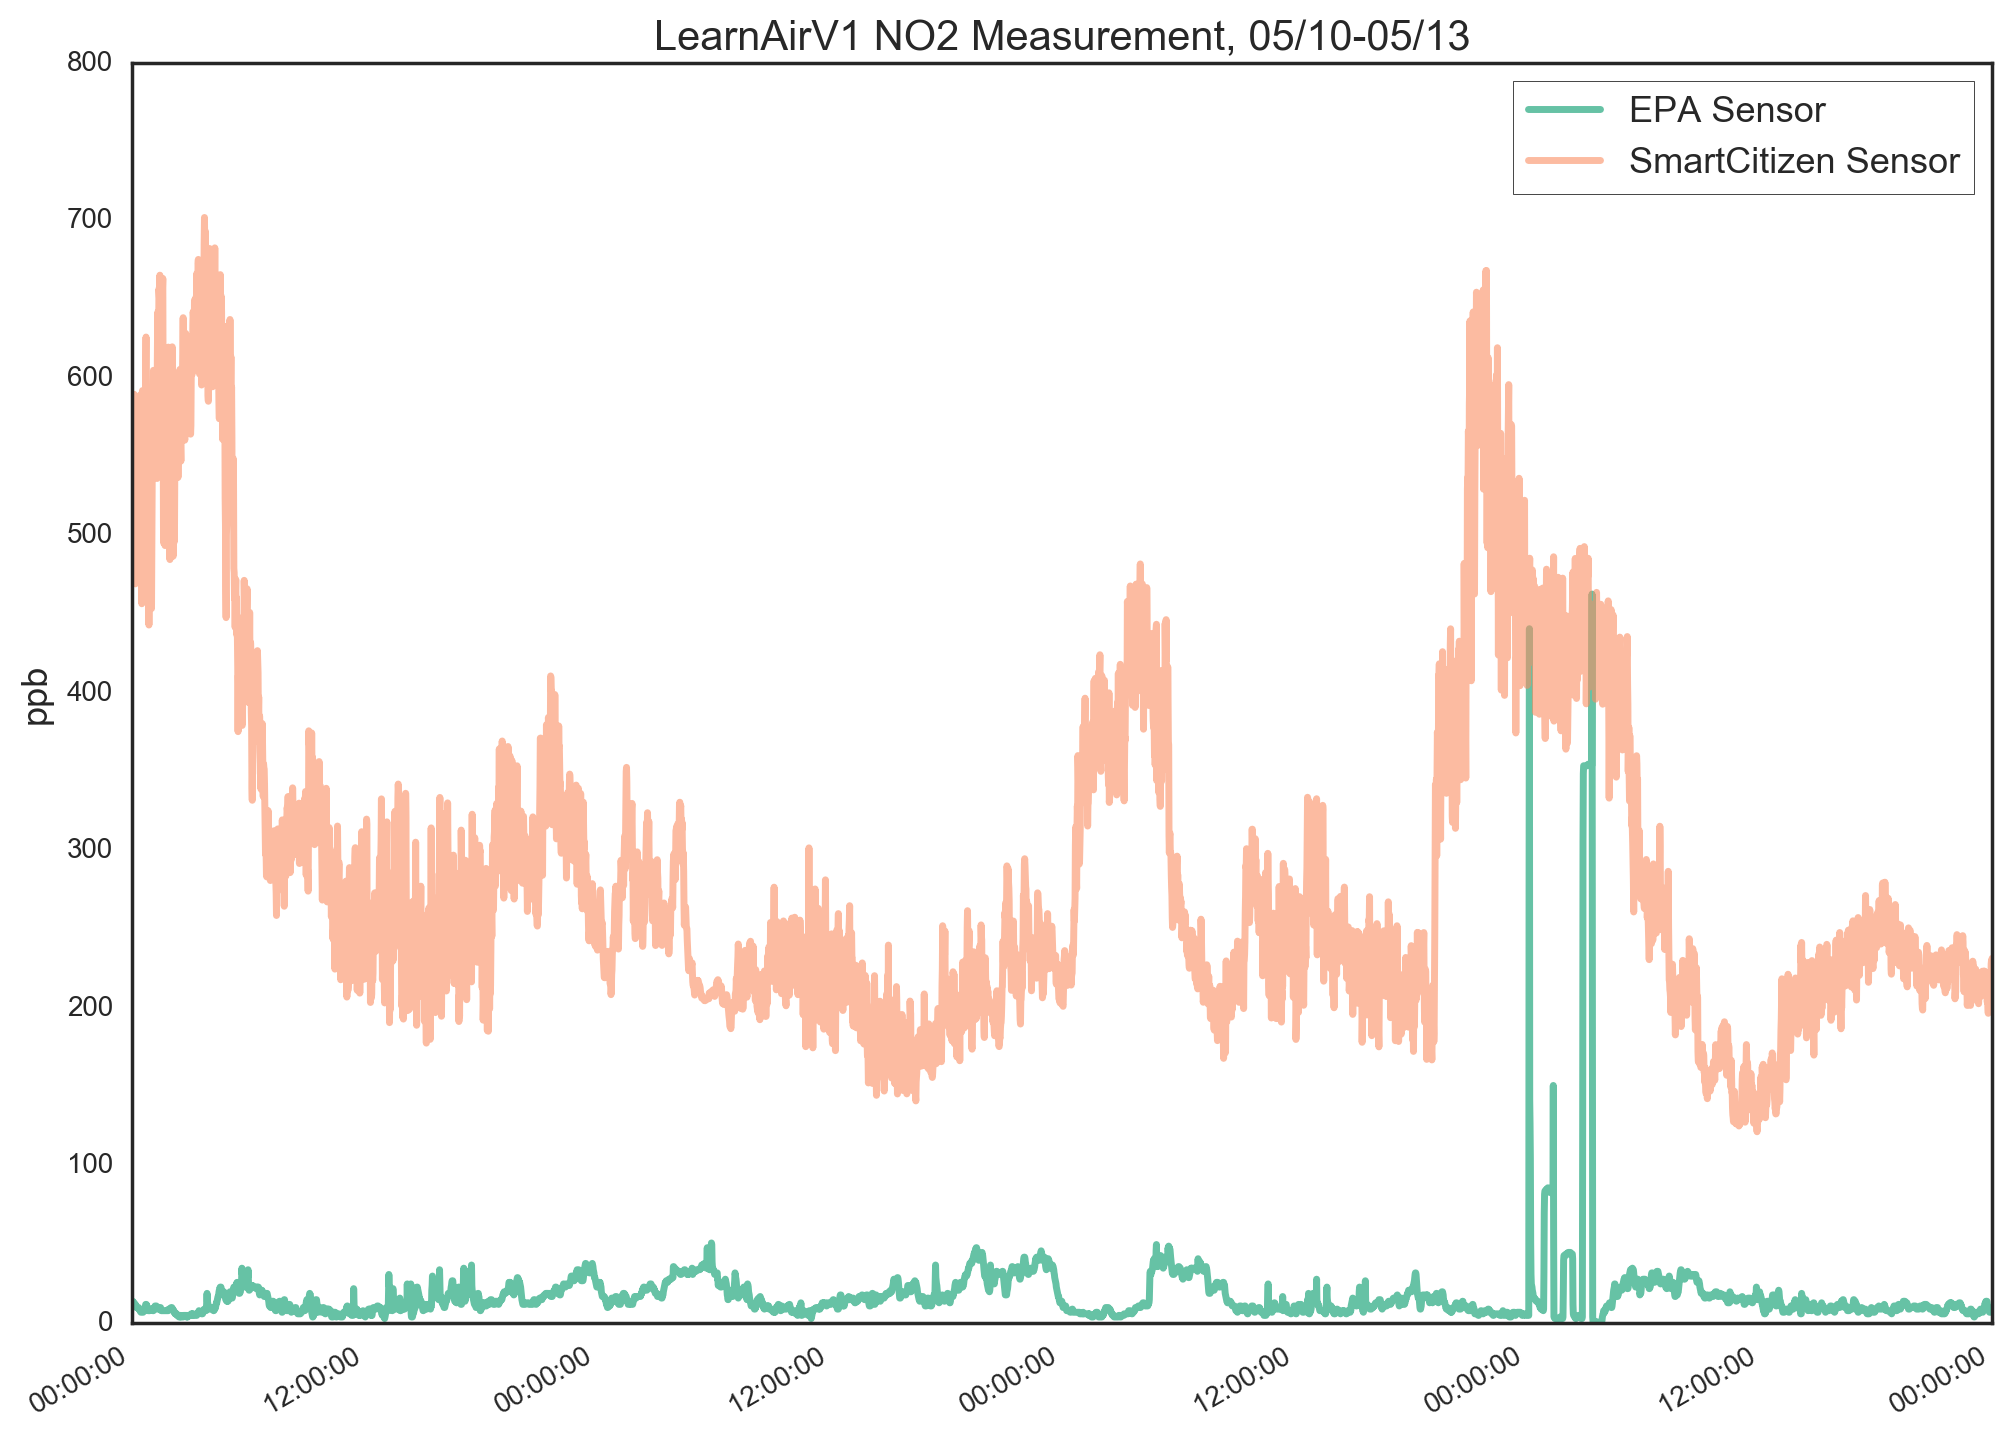
\includegraphics[width=\textwidth]{figs/no2_sck_zoomed}               
 	 \caption{SmartCitizen NO2 Raw Data}
  	\label{fig:sck_no2_raw_zoomed}
\end{marginfigure}

\subsection{Machine Learning}

This case is similar to the SmartCitizen CO sensor, as machine learning will tell us nothing of the sensor's accuracy.  It reduces to a different problem, instead-- predicting NO2 transients and elevated levels based on metrological and other sensor data. 

\begin{figure}[htb]
 	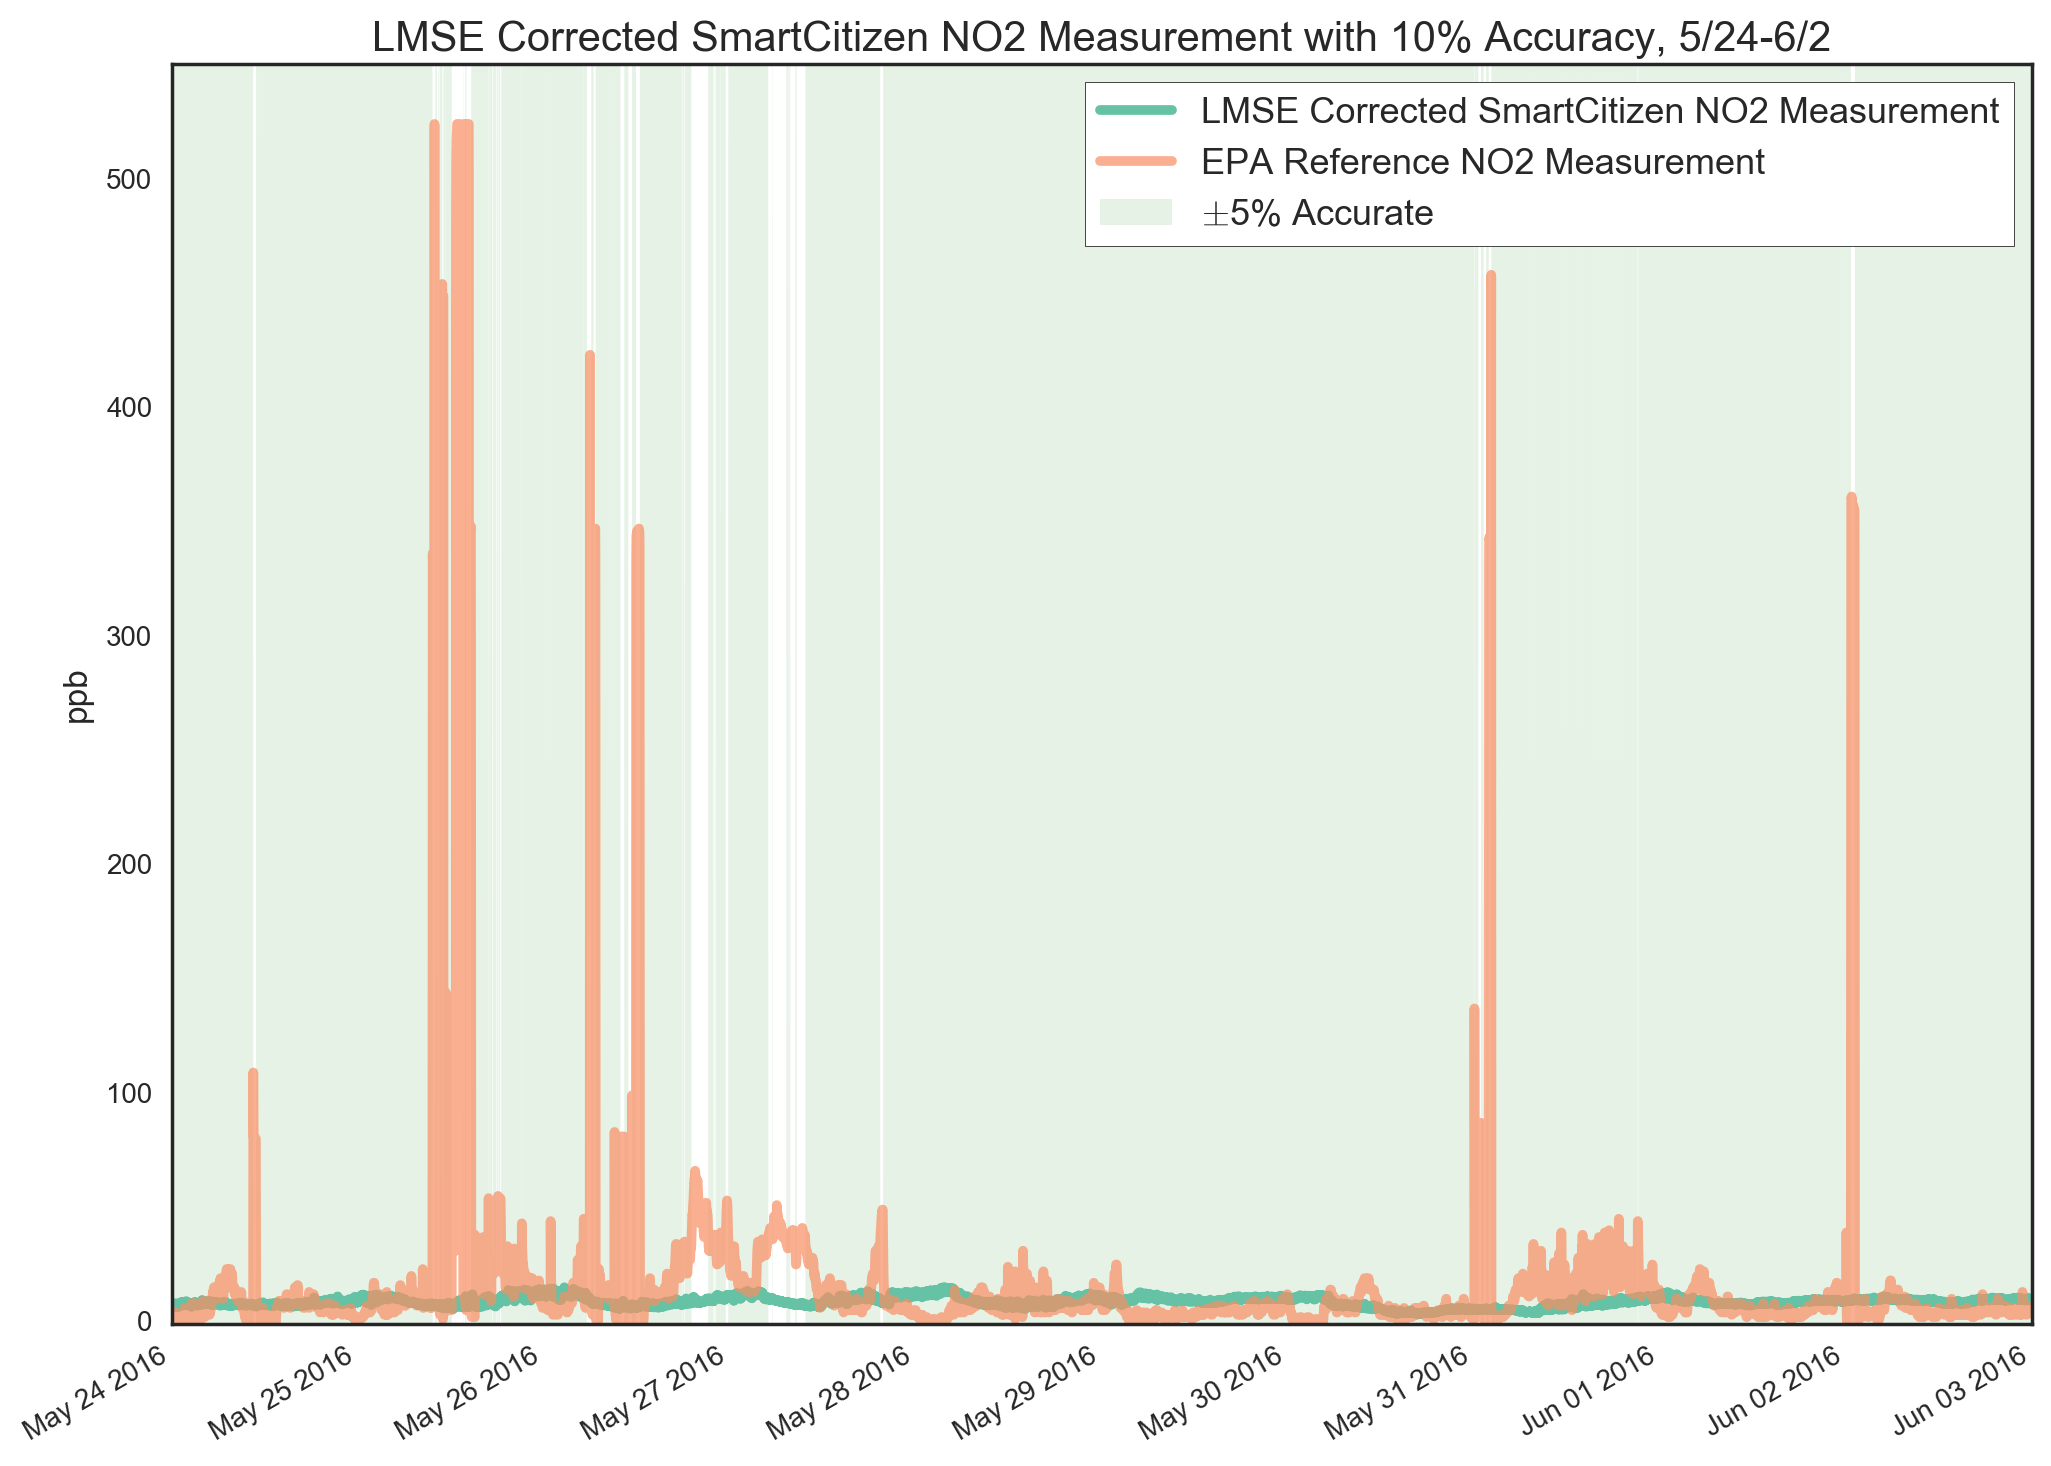
\includegraphics[width=\textwidth]{figs/sck_no2_with_10_accuracy_zoomed}               
 	 \caption{SmartCitizen NO2 with 10\% Accuracy Threshold}
  	\label{fig:sck_no2_with_10_accuracy_zoomed}
\end{figure}



The threshold for accuracy was set at 10\% (or $\pm$5\%) of the full range of values detected for the actual NO2 levels, ~50 ppb ($\pm$25 ppb).   Figure \ref{fig:sck_no2_with_10_accuracy_zoomed} shows the Smart Citizen values against the reference, with `accurate' measurements highlighted with a green background.  The `inaccurate' readings are the peaks and large diversions from the baseline.

As with all of the machine learning models, scikit learn was used to conduct a parameterized search for the optimal logistic regression was conducted using parameters C = [0.001, 0.1, 10, 1000] and penalty-type=['L1', 'L2'] with a 2-fold cross-validation.  An L1 penalty and C=1000 regularization term gave the best ROC\_AUC score of 0.91.  

\begin{table}[]
\centering
\begin{tabular}{|c|c|c|c|c|}
\toprule
\multicolumn{5}{|c|}{Error Rates for SmartCitizen NO2 with Logistic Regression} \\
&\multicolumn{2}{|c|}{all features} & \multicolumn{2}{|c|}{top 15 features} \\
&shuffled & chunked & shuffled & chunked \\
avg & 0.03 & 0.05 & 0.03 & 0.04 \\
min & 0.03 & 0.02 & 0.03 & 0.02 \\
max & 0.03 & 0.08 & 0.04 & 0.06 \\
\bottomrule
\end{tabular}
\label{tab:as1_co_error_rates}
\caption{Error Rates for Predicting SmartCitizen NO2 Accuracy with Logistic Regression}
\end{table}

We see very low error rates of 3-4\% on average with our predictions, regardless of the size of our feature set and whether the validation was randomized or chunked.  This is corroborated by very strong performance in the average confusion matrix (Table \ref{tab:sck_no2_confusion}).  Our ROC curves show tight agreement for the shuffled test sets of 0.90-0.92 AUC-ROC, while the chunked version lags behind slightly with scores from 0.69-0.83.  These results show evidence of extremely strong predictive power, though they hint that we haven't collected quite enough data to completely account for seasonal variation (even though we're doing well enough with the chunked test sets to predict with good confidence).



\begin{figure}[htb]
 	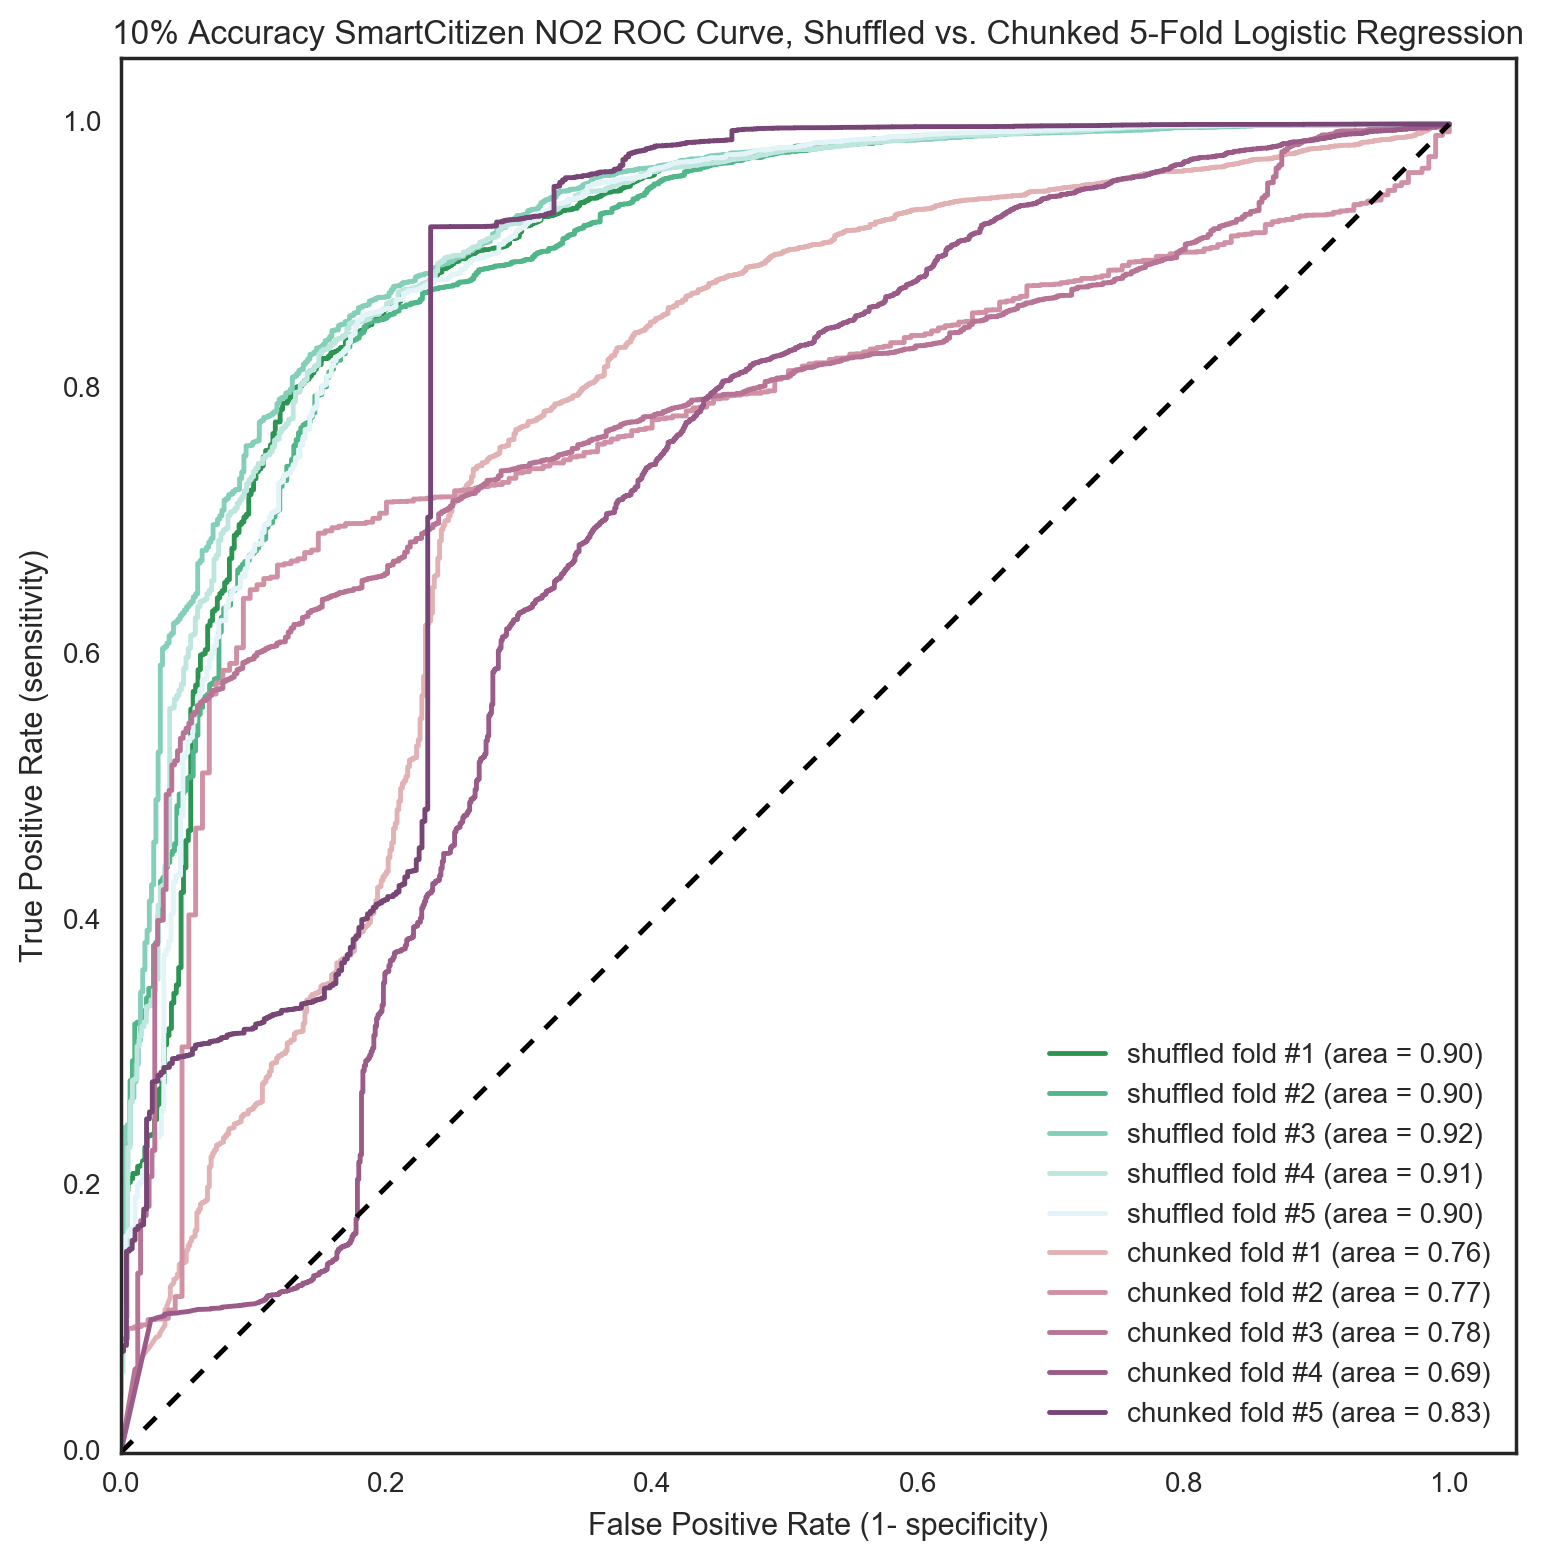
\includegraphics[width=\textwidth]{figs/sck_no2_10_roc}               
 	 \caption{SmartCitizen NO2 ROC Curve}
  	\label{fig:sck_no2_10_roc}
\end{figure}


We see similar error rates with all features as for a subset of the top fifteen.  Examining the AUC-ROC shows that when training only with the top features, the score drops from 0.9 to 0.8 -- a substantial drop, but proof that the top fifteen account for a very strong prediction on their own.
 
The top features are similar to those that predicted the CO transients, but with a stronger relationship-- black carbon is a leading indicator, as well as humidity, the hour of the day, and CO level.  These all make sense as correlates-- CO and black carbon are produced by traffic, which has a predictable pattern with the time of day.  Table \ref{tab:sck_no2_top_features}) shows the top features given seven feature selection algorithms.

\begin{margintable}
\centering
\offinterlineskip
\hspace*{-5cm}\raisebox{-4cm}[0pt][0pt]{\rotatebox[origin=c]{90}{\parbox[c][0pt][c]{3cm}{\textbf{Actual Values}\\[20pt]}}}\par
\hspace{.3cm}\MyHBox[\marginparwidth]{Predicted Values}\par
\vspace{-.5cm}
\hspace*{1cm}\MyHBox{0}\MyHBox{1}\par
\MyTBox{0}{142.0}{427.0}
\vspace{-.35cm}\MyTBox{1}{52.6}{14370.2}\raisebox{-1cm}
}
\label{tab:sck_no2_confusion}
\caption{Average SmartCitizen NO2 Confusion Matrix w/Shuffled K-Fold}
\end{margintable}

Once again, there seems to be strong evidence that NO2 transients are highly predictable if there are other, good quality sensors that measure related phenomena (like black carbon and CO) to rely on.  The relationship is a complex one that requires a larger feature set and a lot of training data for optimal performance, but it appears that even in the short two month period we were able to train a model that would work well under realistic conditions.

\begin{table}[]
\centering
\small
\begin{tabular}{lllllllll}
\\
\\
\toprule
     & Corr. & Lasso & Lin Reg & RF   & RFE  & Ridge & Stability & Mean \\
\midrule
bkcarbon                                   & 1     & 0          & 0    & 1    & 0.63  & 0.51      & 0.85 & 0.57 \\
daily\_avg\_sck\_humidity                  & 0.11  & 0          & 0    & 0.32 & 0.67  & 1         & 0.76 & 0.41 \\
hour\_of\_day                              & 0.07  & 0.92       & 0    & 0.1  & 0.42  & 0.02      & 1    & 0.36 \\
avg\_60\_bkcarbon                          & 0.92  & 0          & 0    & 0.08 & 0.59  & 0.25      & 0.69 & 0.36 \\
derivative\_avg\_1440\_lmse\_calib\_as\_co & 0.06  & 0          & 0    & 0.05 & 0.62  & 0.38      & 1    & 0.3  \\
Solar Panel ( V)                           & 0.03  & 0          & 1    & 0    & 0.88  & 0         & 0    & 0.27 \\
lmse\_sck\_co                              & 0.01  & 1          & 0    & 0.02 & 0.85  & 0         & 0    & 0.27 \\
derivative\_avg\_1440\_bkcarbon            & 0.05  & 0          & 0    & 0.07 & 0.71  & 0.1       & 0.99 & 0.27 \\
humidity\_box\_differential                & 0.02  & 0          & 0.04 & 0.11 & 1     & 0.61      & 0    & 0.25 \\
forecastio\_partly-cloudy-night            & 0.03  & 0          & 0.16 & 0.02 & 0.95  & 0.11      & 0.42 & 0.24 \\
avg\_60\_forecastio\_humidity              & 0     & 0          & 0.04 & 0.06 & 1     & 0.61      & 0    & 0.24 \\
day                                        & 0.07  & 0          & 0    & 0    & 0.97  & 0.05      & 0.51 & 0.23 \\
night                                      & 0.07  & 0          & 0.01 & 0    & 0.98  & 0.05      & 0.43 & 0.22 \\
avg\_60\_forecastio\_precipProbability     & 0.04  & 0          & 0    & 0    & 0.6   & 0.49      & 0.44 & 0.22 \\
daily\_avg\_forecastio\_humidity           & 0.03  & 0          & 0    & 0.05 & 0.66  & 0.48      & 0.24 & 0.21 \\
forecastio\_rain                           & 0.03  & 0          & 0.16 & 0    & 0.9   & 0.25      & 0.04 & 0.2  \\
forecastio\_humidity                       & 0     & 0          & 0    & 0    & 0.64  & 0.72      & 0    & 0.19 \\
forecastio\_clear-night                    & 0.02  & 0          & 0.16 & 0    & 0.93  & 0.03      & 0.1  & 0.18 \\
forecastio\_fog                            & 0     & 0          & 0.16 & 0    & 0.9   & 0.21      & 0    & 0.18 \\
forecastio\_wind                           & 0.01  & 0          & 0.16 & 0    & 0.92  & 0.18      & 0    & 0.18 \\
avg\_720\_bkcarbon                         & 0.47  & 0          & 0    & 0.05 & 0.54  & 0.07      & 0.12 & 0.18 \\
avg\_30\_ws                                & 0.13  & 0          & 0    & 0.08 & 0.45  & 0.02      & 0.48 & 0.17 \\
avg\_15\_derivative\_sck\_temperature      & 0     & 0          & 0    & 0.04 & 0.63  & 0.5       & 0.01 & 0.17 \\
avg\_720\_lmse\_scaled\_sharpDust          & 0.01  & 0          & 0    & 0.16 & 0.58  & 0.41      & 0    & 0.17 \\
\bottomrule
\end{tabular}
\label{tab:sck_no2_top_features}
\caption{Top Features for Predicting SmartCitizen NO2}
\end{table}


